\documentclass[a4paper]{article}
\usepackage[english]{babel}
\usepackage{setspace}
\usepackage{mathtools}
\usepackage{listings}
\usepackage{ulem}
\usepackage[utf8]{inputenc}
\usepackage{eurosym}
\usepackage{amssymb}
\usepackage{fancyhdr}
\usepackage{tikz}
\usepackage{tikzsymbols}
\usetikzlibrary{calc}
\usetikzlibrary{positioning}
\usetikzlibrary{arrows.meta}
\usetikzlibrary{fit}
\usepackage{tikzscale}
\usepackage{wrapfig}
\setcounter{secnumdepth}{-1}
\pagestyle{fancy}
\fancyhf{}
\setlength{\headheight}{24.0pt}
\lhead{Multi-Agent Systems,  Winter Semester 2018/2019, Exercise 3\\
       Submitted by: Amadeus Hovekamp, Hans Nübel, Jonathan Pieper}
\cfoot{\thepage}

\usepackage[
        colorlinks = true,    % Disable drawing boxes around links.
        linkcolor = black,    % Sets the color of links to black.
    ]{hyperref}
\newcommand{\refequation}[1]{\hyperref[#1]{(\ref{#1})}}

\begin{document}
\title{Exercise Sheet 2: Solution}
\author{}
\date{\today}

\section{Exercise 3.1}
\subsection{a)}
\begin{tikzpicture}
\tikzstyle{box}=[rectangle,align=center,draw,text depth=.25ex,line width=0.1mm,fill=white]
\node[box] at(0, 0) (a) {$K(p \lor q) \land K \lnot p$, $K(p \lor q)$, $K \lnot p$,\\
    $p \lor q, \lnot p, p$};
\node[box] at(-1, -2) (b) {$p \lor q$};
\node[box] at(1, -2) (c) {$\lnot p$};
\node[box] at(6, 0) (d) {$K(p \lor q) \land K \lnot p$, $K(p \lor q)$, $K \lnot p$,\\
    $p \lor q, \lnot p, q$};
\draw[<->] (a.south) ++(-1, 0) to (b.north);
\draw[<->] (a.south) ++(1, 0) to (c.north);
\end{tikzpicture}\\
This yields the model $M = (W, R, V)$ with $W = \{w_1\}$, $R(K) = \{(w_1, w_1)\}$, $V(p) = {}$ and $V(q) = \{w_1\}$.


\section{Exercise 3.1 Variation}
\subsection{a)}

\begin{tikzpicture}
\tikzstyle{box}=[rectangle,align=center,draw,text depth=.25ex,line width=0.1mm,fill=white]
\node[box] at(0, 0) (a) {$K\left(p \lor q\right) \land K \lnot p$};
\end{tikzpicture}\\
\\
Apply AND-Rule:\\
\\
\begin{tikzpicture}
\tikzstyle{box}=[rectangle,align=center,draw,text depth=.25ex,line width=0.1mm,fill=white]
\node[box] at(0, 0) (a) {$K\left(p \lor q\right) \land K \lnot p$,\\
                         $K\left(p \lor q\right)$, $K \lnot p$};
\end{tikzpicture}\\
\\
Apply Axiom T:\\
\\
\begin{tikzpicture}
\tikzstyle{box}=[rectangle,align=center,draw,text depth=.25ex,line width=0.1mm,fill=white]
\node[box] at(0, 0) (a) {$K\left(p \lor q\right) \land K \lnot p$,\\
                         $K\left(p \lor q\right)$, $K \lnot p$,\\
                         $p \lor q$, $\lnot p$};
\end{tikzpicture}\\
\\
Apply OR-Rule:\\
\\
\begin{tikzpicture}
\tikzstyle{box}=[rectangle,align=center,draw,text depth=.25ex,line width=0.1mm,fill=white]
\node[box] at(0, 0) (a) {$K\left(p \lor q\right) \land K \lnot p$,\\
                         $K\left(p \lor q\right)$, $K \lnot p$,\\
                         $p \lor q$, $\lnot p$,\\
                         $p$};
\node[box] at(6, 0) (b) {$K\left(p \lor q\right) \land K \lnot p$,\\
                         $K\left(p \lor q\right)$, $K \lnot p$,\\
                         $p \lor q$, $\lnot p$,\\
                         $q$};
\end{tikzpicture}\\
\\
$\bot$-Rule:\\
\\
\begin{tikzpicture}
\tikzstyle{box}=[rectangle,align=center,draw,text depth=.25ex,line width=0.1mm,fill=white]
\node[box] at(0, 0) (a) {$K\left(p \lor q\right) \land K \lnot p$,\\
                         $K\left(p \lor q\right)$, $K \lnot p$,\\
                         $p \lor q$, $\lnot p$,\\
                         $p$,\\
                         $\bot$};
\node[box] at(6, 0) (b) {$K\left(p \lor q\right) \land K \lnot p$,\\
                         $K\left(p \lor q\right)$, $K \lnot p$,\\
                         $p \lor q$, $\lnot p$,\\
                         $q$};
\end{tikzpicture}\\
\\
No more rules can be applied and there is an open premodel left, thus the formula is satisfiable.
Kripke Model: $M = (W, R, V)$ with $W = \{w_1\}$, $R(K) = \{(w_1, w_1)\}$,
              $V(p) = \{\}$ and $V(q) = \{w_1\}$. 
Pointed S5 model $(M, w)$ with M from above and $w=\{\lnot p, q\}$.

\subsection{b)}

\begin{tikzpicture}
\tikzstyle{box}=[rectangle,align=center,draw,text depth=.25ex,line width=0.1mm,fill=white]
\node[box] at(0, 0) (a) {$\lnot \left( K \left(p \land q\right) \rightarrow K p \right)$};
\end{tikzpicture}\\
\\
Apply NotImpl-Rule:\\
\\
\begin{tikzpicture}
\tikzstyle{box}=[rectangle,align=center,draw,text depth=.25ex,line width=0.1mm,fill=white]
\node[box] at(0, 0) (a) {$\lnot \left( K \left(p \land q\right) \rightarrow K p \right)$,\\
                         $\left( K \left(p \land q\right) \land \lnot K p \right)$};
\end{tikzpicture}\\
\\
Apply AND-Rule:\\
\\
\begin{tikzpicture}
\tikzstyle{box}=[rectangle,align=center,draw,text depth=.25ex,line width=0.1mm,fill=white]
\node[box] at(0, 0) (a) {$\lnot \left( K \left(p \land q\right) \rightarrow K p \right)$,\\
                         $\left( K \left(p \land q\right) \land \lnot K p \right)$,\\
                         $K \left(p \land q\right)$, $\lnot K p$};
\end{tikzpicture}\\
\\
Apply Axiom T:\\
\\
\begin{tikzpicture}
\tikzstyle{box}=[rectangle,align=center,draw,text depth=.25ex,line width=0.1mm,fill=white]
\node[box] at(0, 0) (a) {$\lnot \left( K \left(p \land q\right) \rightarrow K p \right)$,\\
                         $\left( K \left(p \land q\right) \land \lnot K p \right)$,\\
                         $K \left(p \land q\right)$, $\lnot K p$,\\
                         $p \land q$};
\end{tikzpicture}\\
\\
Apply AND-Rule:\\
\\
\begin{tikzpicture}
\tikzstyle{box}=[rectangle,align=center,draw,text depth=.25ex,line width=0.1mm,fill=white]
\node[box] at(0, 0) (a) {$\lnot \left( K \left(p \land q\right) \rightarrow K p \right)$,\\
                         $\left( K \left(p \land q\right) \land \lnot K p \right)$,\\
                         $K \left(p \land q\right)$, $\lnot K p$,\\
                         $p \land q$,\\
                         $p, q$};
\end{tikzpicture}\\
\\
Duality:\\
\\
\begin{tikzpicture}
\tikzstyle{box}=[rectangle,align=center,draw,text depth=.25ex,line width=0.1mm,fill=white]
\node[box] at(0, 0) (a) {$\lnot \left( K \left(p \land q\right) \rightarrow K p \right)$,\\
                         $\left( K \left(p \land q\right) \land \lnot K p \right)$,\\
                         $K \left(p \land q\right)$, $\lnot K p$,\\
                         $p \land q$,\\
                         $p, q$,\\
                         $\lnot ( \lnot \hat{K} \lnot p )$
};
\end{tikzpicture}\\
\\
\begin{tikzpicture}
\tikzstyle{box}=[rectangle,align=center,draw,text depth=.25ex,line width=0.1mm,fill=white]
\node[box] at(0, 0) (a) {$\lnot \left( K \left(p \land q\right) \rightarrow K p \right)$,\\
                         $\left( K \left(p \land q\right) \land \lnot K p \right)$,\\
                         $K \left(p \land q\right)$, $\lnot K p$,\\
                         $p \land q$,\\
                         $p, q$,\\
                         $\hat{K} \lnot p$
};
\end{tikzpicture}\\
\\
<l>-Rule





\subsection{c)}

\begin{tikzpicture}
\tikzstyle{box}=[rectangle,align=center,draw,text depth=.25ex,line width=0.1mm,fill=white]
\node[box] at(0, 0) (a) {$\left(K_a p \lor K_a \lnot p \right) \land K_b \left(K_a p \lor K_a \lnot p\right)$};
\end{tikzpicture}\\
\\
Apply AND-Rule:\\
\\
\begin{tikzpicture}
\tikzstyle{box}=[rectangle,align=center,draw,text depth=.25ex,line width=0.1mm,fill=white]
\node[box] at(0, 0) (a) {$\left(K_a p \lor K_a \lnot p \right) \land K_b \left(K_a p \lor K_a \lnot p\right)$,\\
                         $\left(K_a p \lor K_a \lnot p \right)$, $K_b \left(K_a p \lor K_a \lnot p\right)$};
\end{tikzpicture}\\


\subsection{d)}

\begin{tikzpicture}
\tikzstyle{box}=[rectangle,align=center,draw,text depth=.25ex,line width=0.1mm,fill=white]
\node[box] at(0, 0) (a) {$\lnot \left( O \left(O p \rightarrow p \right) \rightarrow \left(O O p \rightarrow O p\right) \right)$};
\end{tikzpicture}\\


\subsection{e)}

\begin{tikzpicture}
\tikzstyle{box}=[rectangle,align=center,draw,text depth=.25ex,line width=0.1mm,fill=white]
\node[box] at(0, 0) (a) {$\lnot \left( O K p \rightarrow O p\right)$};
\end{tikzpicture}\\

\section{Exercise 3.2}
\begin{tabular}{c | c c c c c c}
$\phi$ & $M, w_2 \models$ & $M, w_2 \models$ & $M, w_2 \models$ & $M, w_2 \models$ &
    $M, w_1 \models$ & $M, w_1 \models$\\ 
& $K_1 \phi$ & $K_2 \phi$ & $C \phi$ & $D \phi$ & $C \phi$ & $D \phi$ \\ \hline
$p$ &$\square$&$\boxtimes$&$\square$&$\boxtimes$&$\square$&$\square$\\
$q$ &$\boxtimes$&$\square$&$\square$&$\boxtimes$&$\square$&$\boxtimes$\\
$p \land q$ &$\square$&$\square$&$\square$&$\boxtimes$&$\square$&$\square$\\
$p \lor q$ &$\boxtimes$&$\boxtimes$&$\boxtimes$&$\boxtimes$&$\boxtimes$&$\boxtimes$
\end{tabular}\\

\end{document}
